In this chapter we will give a motivation for this thesis.\footnote{There are \emph{other} motivations, i.e.\ other concepts that \emph{perfect tangles} can be seen as a generalization of. We will see this in the next chapters.} We will define \emph{absolutely maximally entangled states} (AME states), and extract the notion of a \emph{planarly perfect tensor} from that definition. A few applications of both of these concepts will be listed --- the purpose of this this thesis is not to give a detailed description of these concepts, but rather generalize them in a specific way. Detailed accounts of both AME states, perfect tensors, and how they are used can be found in the literature referenced throughout this chapter.

After that, we will talk a bit about the \emph{Temperley-Lieb algebras}, one of the most important foundational concepts for this thesis. Most calculations and generalization are made or explained using these algebra, more specifically their nice graphical calculus.

\section{AME States}
Absolutely maximally entangled states (AME states) have been around for a while, and have, thanks to their high degree of entanglement, found applications in e.g.\ the the construction of quantum error correcting codes \cite{raissi2017constructingQECC}. 

The basic idea is that they are multipartite states such that for any bipartition of the system, tracing out the bigger subsystem yields the maximally mixed state, i.e.\ the two subsystems in the bipartition are maximally entangled. The precise definition is stated in this section.

\bigno Suppose we have a system of $n$ qudits, so that the system Hilbert space looks like 
\begin{align*}
\mathcal{H}\cong \bigotimes_{i=1}^n \mathcal{H}_i,
\end{align*}
with single qudit spaces $\mathcal{H}_i\cong \mathbb{C}^d$. 

By a \emph{bipartition} of this system we mean the following. Take any subset $A$ of $I=\{1, \ldots, n\}$, the set of indices. From this we get a bipartition of $I$, namely $I=A\cup A^c$. We can then define a subspace 
\begin{align*}
\mathcal{H}_A\equiv\bigotimes_{i\in A}\mathcal{H}_i,
\end{align*}
and $\mathcal{H}_{A^c}$ analogously, so that we can now partition the whole system: $\mathcal{H}\cong \mathcal{H}_{A}\tensor\mathcal{H}_{A^c}$. This is all we need to define these peculiar states.

\begin{definition}[AME State]\index{Absolutely maximally entangled state}
A state $|\psi\rangle\in\mathcal{H}$ is called an \emph{AME state} iff for any bipartition $I=A\cup A^c$ with $\lvert A \rvert \leq \lvert A^c \rvert$ it is true that
\begin{align*}
\mathrm{tr}_{A^c} |\psi\rangle\langle\psi| = \frac{1}{d^{\lvert A \rvert}}\mathbf{1}_{A}.
\end{align*}
Here $\mathrm{tr}_{A^c}$ denotes the partial trace over the subsystem $\mathcal{H}_{A^c}$, and $\mathbf{1}_A$ is the identity on $\mathcal{H}_A$.
\end{definition}
The condition `$\lvert A \rvert \leq \lvert A^c \rvert$' in this definition is equivalent to $\lvert A \rvert\leq\floor{\frac{n}{2}}$, and it is there to ensure that we trace out the bigger subsystem --- otherwise, getting the maximally mixed state would not even be possible.

In general the conditions (on a given system) that guarantee the (non)existence of AME states are not clear \cite{raissi2017constructingQECC}.\footnote{
A pretty big table stating whether AME states exist for given local dimension $d$ and qudit number $n$ can be found at \url{http://web.archive.org/web/20171004134422/http://www.tp.nt.uni-siegen.de/+fhuber/ame.html} (archived on 04.10.2017)
} That they exists, however, is out of the question: Clearly the \emph{Bell states}, i.e.\ maximally entangled states of two qubits ($n=2$, $d=2$), are by definition trivially AME. Another example is the \emph{Greenberger-Horne-Zeilinger} (qubit) state
\begin{align*}
|GHZ\rangle_3 = \frac{1}{\sqrt{2}} \left( |000\rangle+|111\rangle \right),
\end{align*}
and it is easy to see that this satisfies the definition of an AME state: the condition imposed on the size of $A$ implies that we are to trace out any two-qubit subsystem, and clearly, then, the result is ${}^1/_2$ the identity on $\mathbb{C}^2$. 

While more easy and not-so-easy examples exist, it is not necessary to present them here, as we are more interested in the conceptual side for now.

\section{Perfect Tensors}
Although \emph{perfect tensors} themselves do not rely on the definition of AME states, we will here go the same route as \cite{raissi2017constructingQECC}, and
show that the concept of a perfect tensor emerges from that of AME states.

\bigno
Let $|\psi\rangle$ be an AME state in any $n$-qudit system. We can choose a computational basis of $\mathcal{H}\cong\mathbb{C}^{d^n}$ and write $\ket{\psi}$ as
\begin{align*}
\ket{\psi} = c_{j_1 \cdots j_n} \ket{j_1 \cdots j_n}, c_{j_1 \cdots j_n}\in\mathbb{C},
\end{align*}
where summation over repeated indices is implied. Suppose now, without loss of generality, that we have a bipartition with $A=\{1, \ldots, m\},$ $m\leq n$. (We are taking this bipartition because it then is easier to see what's happening. It is clear how to generalize this to arbitrary bipartitions with $A$ smaller than $A^c$.)

Using this, we may write
\begin{align*}
\ket{\psi} &= \ket{j_1\cdots j_m} \tensor \left( c_{j_1 \cdots j_n} \ket{j_{m+1}\cdots j_n}\right) \\
&\equiv \ket{j_1\cdots j_m} \tensor C\ket{j_1\cdots j_m},
\end{align*}
thus defining a linear map $C  :\mathcal{H}_A \rightarrow \mathcal{H}_{A^c}$ via
\begin{align}\label{eq:mapfrombipartition}
C \equiv c_{j_1 \cdots j_n} \ket{j_{m+1}\cdots j_n} \bra{j_1\cdots j_m},
\end{align}
i.e.\  a matrix with components indexed by basis vectors $\vec{j}\in\mathcal{H}_A$ and $\vec{J}\in\mathcal{H}_{A^c}$, $C=C_{\vec{j}\vec{J}}\ket{\vec{J}}\bra{\vec{j}}$.

So far, we have not invoked the fact that $\ket{\psi}$ is AME. But watch what happens when we trace out $\mathcal{H}_{A^c}:$
\begin{align*}
\mathrm{tr}_{A^c} |\psi\rangle\langle\psi|  
=& \ket{\vec{j}} \bra{\vec{j^\prime}}    \cdot   \bra{\vec{j^\prime}}C^\dagger C\ket{\vec{j}}.
\end{align*}
Given that $\ket{\psi}$ is AME, this must be equal to the maximally mixed state. Clearly this is possible if and only if $C^\dagger C$ is proportional to the identity on $\mathcal{H}_A$.

And, coincidentally, this is equivalent to the definition of \emph{perfect tensor} given in \cite{Pastawski2015Holographic}: A tensor with the property that, whenever possible, certain associated maps are (proportional to) isometries. To see this we must first be on one page about what a \emph{tensor} is.

\begin{definition}[Tensor]\label{def:tensor}\index{Tensor}
An \emph{$n$-leg tensor} is a set of (complex) numbers indexed by $n$ copies of an indexing set $J$. The \emph{range} of an index is the number $\lvert J \rvert$,\footnote{In the present setting this is sufficient. More generally, one could require the number to be index by $n$ indexing sets, but this is not necessary here. The range of the $i$th index would then be the size of the $i$th indexing set.} and we commonly call the indices \emph{legs}.
\end{definition}
Clearly, then, the set of coefficients of the AME state $\ket{\psi}$ is an  $n$-leg tensor, and the indexing set is $J=\{1, \ldots, d\}$: The legs correspond to single qudits, and the indexing set is actually a basis for $\mathbb{C}^d$. 

In particular, any $n$-leg tensor whose legs range from $1$ to $d$ can be seen as a vector in $\mathbb{C}^{d^n}$. But we can also interpret such a tensor as the coefficients of a linear map $T$ between complex vector spaces such that 
\begin{align*}
\dim\mathrm{dom~} T + \dim\mathrm{codom~} T = d^n.
\end{align*}
We make this precise in the following proposition.

\begin{proposition}\label{prop:tensorAME}
Let $C=\{C_{j_1\cdots j_n}\}$ be an $n$-leg tensor, with indices ranging from $1$ to $d$, and let $\mathcal{H}$ be any $n$-qudit Hilbert space like above. Then the following are equivalent (up to normalization).
\begin{itemize}
\item[\text{(i)}] The $n$-qudit state defined by 
\begin{align*}
C_{j_1\cdots j_n}\ket{j_1\cdots j_n}
\end{align*}
is an AME state.
\item[(ii)] For any bipartition $A\cup A^c$ of $\{1,\ldots, n\}$ with $\lvert A \rvert\leq \lvert A^c \rvert$ the linear map
\begin{align*}
C^{A\to A^c} : \mathcal{H}_A \rightarrow\mathcal{H}_{A^c}
\end{align*}
defined by (sums implied)
\begin{align*}
C^{A\to A^c}\equiv C_{j_1\cdots j_n} \ket{j_i}_{i\in A^c}\bra{j_l}_{l\in A}
\end{align*}
is proportional to an isometry, or, equivalently, 
\begin{align*}
\left(C^{A\to A^c}\right)^\dagger C^{A\to A^c} \propto \mathbf{1}_{\mathcal{H}_A}
\end{align*}
\end{itemize}
\begin{proof}
$(i)\implies (ii)$ is clear by definition.

 Likewise, $(ii)$ implies $(i)$ up to normalization, as we have already established, so this is clear once we have shown the equivalence appearing within $(ii)$, namely that a linear map $T$ being proportional to an isometry is equivalent to $T^\dagger T$ being proportional to the identity. But this, again, is easy.
Suppose the latter. Then, for $a,b\in\mathrm{dom~}T$,
\begin{align*}
\langle a, b\rangle \propto \langle a, T^\dagger T b \rangle = \langle Ta, Tb \rangle,
\end{align*}
so $T$ is proportional to an isometry. Conversely, an isometry is injective, that is, bijective onto its image. So if $T=\alpha S$, where $\alpha\in \mathbb{C}$ and $S$ is an isometry, then $T^\dagger T = \lvert \alpha \rvert^2 S^\dagger S = \lvert \alpha \rvert^2 \mathbf{1}$.
\end{proof}
\end{proposition}

\bigno
Enter perfect tensors. The whole point of them is to be able to use them for constructing certain \emph{tensor networks} with specific properties --- what exactly this means will be clarified in the next subsection, after the definitions.

\begin{definition}[Perfect Tensor]
A tensor associated to an AME state like in the previous proposition is called a \emph{perfect tensor}.
\end{definition}

In this thesis, we will not be needing the full power of the theory of \emph{holographic codes}, so we use a more general notion where we don't take all bipartitions into account. 

To start off with, we need to know what a \emph{connected bipartition} is. Given a set $I=\{1,\ldots, n\}$, a connected bipartition of this set is a bipartition $A\cup A^c=I$ s.t.\ $A$ consists of subsequent numbers, modulo $n$. As an example, if $n=3$, then this is true for every bipartition, but if $n=4$, then the bipartition $\{1,3\}\cup\{2,4\}$ is not connected, while $\{1,4\}\cup\{2,3\}$ surely is.

We then can define tangles that are perfect but not quite, and we will call them \emph{planarly perfect tensors} for now. 

\begin{definition}[Planarly Perfect Tensor]\label{def:planarly perfect tensor}\index{Tensor!Planarly Perfect}
An $n$-leg tensor $T=\{T_{j_1\cdots j_n}\}_{j_i=0}^d\subset\mathbb{C}$ is \emph{planarly perfect} if for any connected bipartition of its legs, say $A\cup A^c$, with $\lvert A \rvert\leq \floor{\frac{n}{2}}$ the associated map
$T^{A\rightarrow A^c}$, as defined in the preceding proposition,
is proportional to an isometry.
\end{definition}
Clearly then, any perfect tensor is also planarly perfect. But the converse is false in general. And since in this thesis we are not interested in perfect tensors but only in the `planar' version, we will simply call those \emph{perfect tensors} from now on.

%The second part of this proposition is the definition of \emph{perfect tensor} given in e.g.\ \cite{Pastawski2015Holographic} and \cite{Osborne:2017woa}. In the following it will be more convenient to work with this definition --- we only wanted to showcase the connection between AME states and perfect tensors after all.

\subsection*{Tensor Networks}
We will now review some of the basics of the tensor network formalism, but not more than we shall need. This will make clear why we are only taking \emph{connected bipartitions} into consideration: Diagrams remain embedded in $\mathbb{R}^2$.

Since we will not need to use the full power of the formalism we refer to \cite{TN_orus, TN_biamonte} for a more in-depth introduction and further applications.

\bigno
The language of tensor networks is of pictorial nature: An $n$-leg tensor $T$ is represented as a `blob' or vertex, labeled $T$, with $n$ lines protruding from it, as seen in \figref{fig:tensor_penrose_notation_example}. The lines will unsurprisingly be called \emph{legs}. One interval between two legs on the boundary of the blob is marked with a $\markedPoint$, indicating that the leg to its left is the first tensor index, giving us an enumeration of the indices in a counterclockwise fashion with a given starting point.

\begin{figure}[!htp]\centering
	\begin{tikzpicture}[scale=0.8]
		\coordinate (center) at (0,0);
		\node (T) at (center) {$T$};
		\draw (center) circle (3mm);
		\foreach \x in {1,2,3}
			\draw ($(center) + (-30 + 120*\x:3mm)$) -- ($(center) + (-30+120*\x:10mm)$) node[above]{\tiny$j_\x$};
		\node (star) at ($(center) + (45:5mm)$) {$\markedPoint$};
	\end{tikzpicture}
	\caption{A 3-leg tensor}
	\label{fig:tensor_penrose_notation_example}
\end{figure}

Obviously here the direction of the legs has no significance. But, as we have seen before, we can build (multi)linear maps from these tensors --- how do we depict this? First recall that each leg lives in its own Hilbert space: It is then clear that only maps coming from connected planar bipartitions, i.e.\ bipartitions of the legs where each set consists of adjacent legs only, make sense in planar pictures.

For the 3-leg tensor $T$ we could for example build the map $T_{j_1j_2j_3}\ket{j_2j_3}\bra{j_1}$, and draw a slightly different picture which is read from bottom to top:

\begin{align*}
	\begin{tikzpicture}[scale=0.8]
		\node[draw,circle,inner sep=0.3mm] (T) at (0,0) {$T$}; 
		\node (star) at ($(T) - (45:5mm)$) {$\markedPoint$};
		\draw (T.south) -- ($(T.south) + (0,-0.6)$) node[right]{\tiny $j_1$};
		\draw (T.50) -- ($(T.50)+ (0,0.6)$) node[right]{\tiny $j_2$};
		\draw (T.130) -- ($(T.130) + (0,0.6)$) node[left]{\tiny $j_3$};		
	\end{tikzpicture}
\end{align*}

Thus it is easily seen that any $n$-leg tensor can be interpreted as a vector, i.e.\ a \emph{ket} in some Hilbert space with $n$ tensor factors, by simply having all legs go up. It is then natural to ask whether a \emph{bra} is obtained by having all legs point down. This does not quite work, since the legs are still numbered from $\markedPoint$ on clockwise. This is a problem because we should be able to contract tensors along common indices, and, in particular, we would like to have the notion of an inner product in the graphical notation.

\bigno So let us digress and talk about what contraction along common indices should be. If $T=\{T_{j_1\cdots j_n}\}$ and $S=\{S_{j^\prime_1\cdots j^\prime_{m}}\}$ are tensors whose legs have range $d$, then we can build for example the following $(n+m-2)$-leg tensor by contracting along, say, the common index $j^{\phantom{\prime}}_{i^{\phantom{\prime}}}=j^\prime_{i^\prime}$
\begin{align*}
\left\{\delta_{j^{\phantom{\prime}}_{i^{\phantom{\prime}}} j^\prime_{i^\prime}} T_{j^{\phantom{\prime}}_1\cdots j^{\phantom{\prime}}_n}S_{j^\prime_1 j^\prime_{m}}  \right\},
\end{align*}
where $\delta_{kl}$ is the Kronecker delta and summation over repeated indices is implied.

Contraction translates to the pictures as in the following example. If we take $T$ and $S$ to both be the 3-leg tensor from \figref{fig:tensor_penrose_notation_example}, and we contract along $j_1$, then we simply connect the $j_1$ legs of both tensors: connected legs imply summation over the associated index. We can see this in \figref{fig:tensor contraction example}.

\begin{figure}[!htp]\centering
	\begin{minipage}{0.8\textwidth}\centering
		\begin{tikzpicture}[scale=0.8]
			\coordinate (center) at (0,0);
			\coordinate (abovecenter) at ($(center) + (0,2)$);
			\node (T) at (center) {$T$};
			\node (T2) at (abovecenter){$T$};
			\draw (center) circle (3mm);
			\draw (abovecenter) circle (3mm);
			\foreach \x in {1,2,3}{
				\draw ($(center) + (-30 + 120*\x:3mm)$) -- ($(center) + (-30+120*\x:10mm)$);
				\draw ($(abovecenter) + (30 + 120*\x:3mm)$) -- ($(abovecenter) + (30 + 120*\x:10mm)$);
				}
			\node (star) at ($(center) + (45:5mm)$) {$\markedPoint$};
			\node (star) at ($(abovecenter) + (225:5mm)$) {$\markedPoint$};
		\end{tikzpicture}
		\caption[Tensor contraction]{Contraction along a shared index. This tensor is not yet interpreted as vector or map.}\label{fig:tensor contraction example}
	\end{minipage}
\end{figure}

\bigno
So how to define `dual diagrams' now? By thinking about Hilbert spaces, we gather that a dual vector should be obtained by an operation $\dagger$ that we are yet to define for pictures. We consider a two leg tensor $v$, build the ket $\ket{v}$ from it, and then deduce from the scalar product of $T$ with itself what $\bra{v} = \ket{v}^\dagger$ might look like as a diagram. 

We have $\ket{v} = v_{j_1j_2}\ket{j_1j_2}$
and
\begin{align*}
\langle v|v \rangle = \overline{v}_{i_1i_2} v_{j_1j_2}\langle i_1i_2|j_1j_2 \rangle = \overline{v}_{j_1j_2} v_{j_1j_2}.
\end{align*}
If we draw this as a diagram it actually looks like this: 
\begin{align*}
\langle v|v \rangle =\,
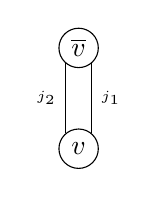
\begin{tikzpicture}[scale=0.8, baseline]
	\node[draw, circle, inner sep=0.3mm, minimum size=0.5cm] (T) at (0,-0.8) {$v$};
	\node[draw, circle, inner sep=0.3mm, minimum size=0.5cm] (Tadj) at (0,0.8) {$\overline{v}$};
	\draw (T.50) -- node[right]{\tiny $j_1$} (Tadj.310);
	\draw (T.130) --  node[left]{\tiny $j_2$} (Tadj.230);
\end{tikzpicture},
\end{align*}
where $\overline{v}$ is the set obtained by complex conjugating every element in the set $v$.

In addition, not only do the legs point down, but their order has been reversed, i.e.\ they are now labeled following the mathematical negative direction. We conclude that the operation $\dagger$ is mirroring in a horizontal line and taking complex conjugates, and this is exactly how it is defined for general tensors.

\bigno This is a step towards defining perfect tensors directly via the graphical calculus, and we have almost understood the defining property, i.e.\ being proportional to an isometry. To fully understand what's going on we only need to invoke the fact from part $(ii)$ of \textsf{Proposition \ref{prop:tensorAME}}, and think about what the identity might be, graphically.

But this is quite easy. For example, on the Hilbert space $\mathcal{H}$ spanned by the legs of an $n$-leg tensor, we have
\begin{align*}
\mathbf{1}_{\mathcal{H}} = \delta_{j^{\phantom{\prime}}_1 j^\prime_1} \cdots \delta_{j^{\phantom{\prime}}_n j^\prime_n} \ket{j^{\phantom{\prime}}_1\cdots j^{\phantom{\prime}}_n}\bra{j^\prime_1 \cdots j^\prime_n},
\end{align*}
each $j_i$ ranging over $d$ values, giving us a $2n$-leg tensor. From the definition it is clear how this acts on an $n$-leg tensor $T=\{T_{j_1\cdots j_n}\}$ when contracting $n$ legs: Trivially. That is, it does not change the tensor $T$ at all. We then simply represent this as $n$ lines, with a label $j_i$ attached to the $i$th line. Contraction with the identity is then nothing more than `elongating the legs'.
\bigno
\begin{remark}
There exists a natural \emph{tensor/monoidal product} for these diagrams, given by drawing two pictures next two each other, e.g.\ a straight line next to a straight line is the identity on the tensor product of the spaces associated with the lines. 

Multiplying a tensor diagram by a number $c$ is the same as multiplying each element of the set defining that tensor by $c$.
\end{remark}

\bigno An $n$-leg tensor is by definition perfect if contracting any connected combination of at least $\ceil{\frac{n}{2}}$ legs with the corresponding legs of the adjoint yields something proportional to the identity (on the space spanned by the uncontracted legs, that is). As an example we evoke our trusty companion, the 3-leg tensor $T$. It is perfect iff
\begin{center}
	\begin{tikzpicture}[scale=0.8, minimum size=6mm]
		\node[draw,circle,inner sep=0.4mm] (T) at (0,0) {$T$}; 
		\draw (T.south) -- ($(T.south) + (0,-0.6)$) node[right]{\tiny $j_{i_1}$};
		\draw (T.50) -- ($(T.50)+ (0,0.3)$) node[right]{\tiny $j_{i_2}$};
		\draw (T.130) -- ($(T.130) + (0,0.3)$) node[left]{\tiny $j_{i_3}$};	
%		
		\node[draw,circle,inner sep=0.4mm] (Tdag) at ($(T |- T.130)+(0,0.8)$) {$\overline{T}$}; 
		\draw (Tdag.north) -- ($(Tdag.north) + (0,0.6)$) node[right]{\tiny $j_{i_1}$};
		\draw (Tdag.230) -- ($(T.130)+ (0,0.3)$);
		\draw (Tdag.310) -- ($(T.50) + (0,0.3)$);
		\node (propto) at (1.5,0.5) {$\propto$};
		\draw ($(T.south) + (2.3,-0.6)$) -- ($(Tdag.north) + (2.3,0.6)$);
	\end{tikzpicture}
\end{center}
for all distinct $i_1, i_2, i_3 \in \{1,2,3\}$. Note that may also decorate the node representing the adjoint with $T^\dagger$ or $T^*$. This does not cause confusion.

\bigno We will now define what a tensor network is. To this end let us first state the definition of an \emph{open graph}: a graph is open iff it is a graph that also has edges one end of which is not at a vertex. For example, \tikz[scale=0.8, baseline=-1mm]{\node[draw, circle, fill, inner sep=0.4mm] (c) at (0,0) {}; \draw (c) -- (0.8,0);} is an open graph with one (open) edge and one vertex. We will also speak of the \emph{degree} $\mathrm{deg}(v)$ of a vertex $v$, which is simply the number of edges attached to it.

\begin{definition}[Tensor Network]
Consider a planar graph $G$, not necessarily open, and not necessarily simple. A \emph{tensor network} (on $G$) is the following data.

To each vertex $v$ assign a $\mathrm{deg}(v)$-leg tensor $T_v$, with some choice of $\markedPoint$ --- the legs of the tensor are then either open edges, or edges to some other vertex $v^\prime$. Since $G$ is not necessarily simple there may be more than one edge connecting $v$ and $v^\prime$ and we record this fact by means of an index, i.e.\ denoting it $(v, v^\prime)_i$, thereby enumerating all edges between $v$ and $v^\prime$. We didn't assume $G$ to be directed, so let us additionally stipulate that $(v, v^\prime)_i = (v^\prime, v)_i$.
 
Thus, we must also impose an obvious compatibility condition: It must be possible to contract $T_v$ and $T_{v^\prime}$ along all of their shared legs, i.e.\ $(v, v^\prime)_i$ for all $i$.
\end{definition}
But what is a tensor network? The immediate interpretation is fairly simple. On a graph with one vertex and $n$ open edges, a tensor network is simply an $n$-leg tensor. And indeed, the generalization is true: A tensor network with $n$ open edges can readily be interpreted as an $n$-leg tensor, by simply contracting all internal edges, i.e.\ edges that are not open\footnote{We should remark that the order in which we contract is crucial when the aim is computational efficiency, see \cite[p.\ 10]{TN_orus}. But this does not really play a role in the scope of this thesis.}, and if $n$ is even, a tensor network can in particular be interpreted as a state, up to normalization (assuming all open edges are legs with the same \emph{local dimension}, i.e.\ range).

\subsection*{Tensor Networks as a Toy Model for the Holographic Correspondence}
The importance of tensor networks built in a certain way using only a perfect tensor was discovered by \cite{Pastawski2015Holographic}. To better understand the proposed AdS/CFT-duality --- a connection between a $(d+1)$-dimensional gravitational theory and a $d$-dimensional conformal field theory `living on the boundary' of spacetime --- the authors derived sort of a discretized toy model in $2+1$ dimensions. 

$\text{AdS}_{2+1}$ is a solution to Eintein's field equations with constant negative curvature, and we may envision it as a solid cylinder, with the temporal axis along its length. Spacial slices, i.e.\ spacelike submanifolds at fixed time, are copies of 2-dimensional hyperbolic space. 

\begin{figure}[!htp]\centering
\begin{minipage}{0.8\textwidth}\centering
	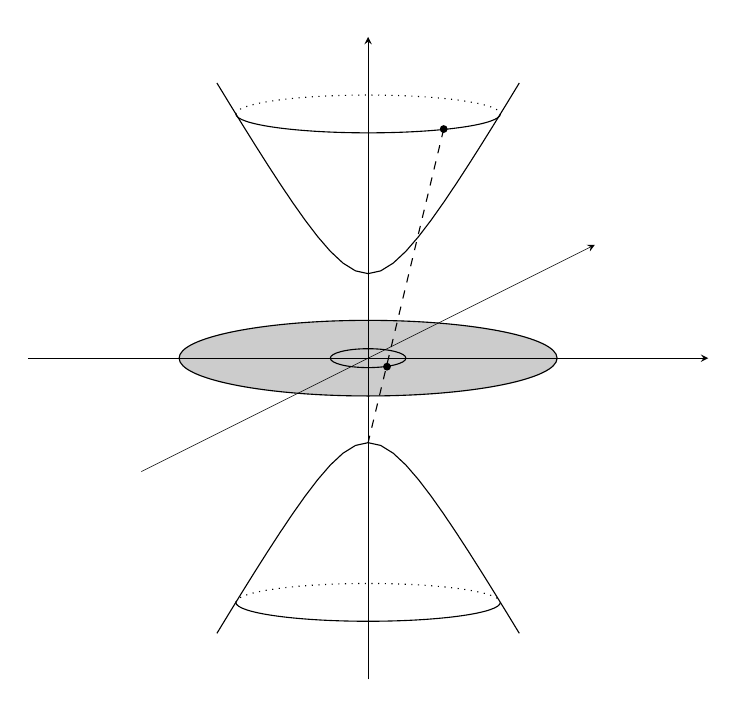
\begin{tikzpicture}[scale = 2.4]
		\draw[fill, color=gray!40] (0,0) circle [x radius = 1cm, y radius = 0.2cm];
		\draw[->, >=stealth, line width= 0.2pt] (-1.8,0) -- (1.8,0) node {};
		\draw[->, >=stealth, line width= 0.2pt] (0,-1.7) -- (0,1.7) node {};
		\draw[->, >=stealth, line width= 0.2pt] (-1.2,-0.6) -- (1.2,0.6) node {};
		\draw (0,0) circle [x radius = 1cm, y radius = 0.2cm];
		\draw[domain = -0.8:0.8] plot (\x, {sqrt(3*\x * \x+ 0.2)});
		\draw[domain = -0.8:0.8] plot (\x, {-sqrt(3*\x * \x+ 0.2)});
		\draw[dashed]  (0.4, {sqrt(3*0.7 * 0.7+ 0.2)-0.08}) node[circle, fill,inner sep=1pt] {}-- (0, {-sqrt(0.2)});
		\foreach \x in {-1, +1}{
			\draw (-0.7, {\x*sqrt(3*0.7 * 0.7+ 0.2)}) arc (180:360:0.7cm and 0.1cm);
			\draw[dotted] (-0.7, {\x*sqrt(3*0.7 * 0.7+ 0.2)}) arc (180:0:0.7cm and 0.1cm);
		}
		\draw (0,0) circle [x radius= 0.2cm , y radius= 0.05cm];
		\node[circle, fill, inner sep=1pt] (bla) at (0.1,-0.045) {};
	\end{tikzpicture}
	\caption[Hyperbolic stereographic projection]{Stereographic projection of a circle on the upper hyperbolic sheet onto a circle in the disk (grey). The inner circle is just supposed to represent the image of the curve in the upper sheet.} % This image is almost a direct copy of the one in \cite{lee1997riemannian}
	\label{fig:Poincare disk construction}
\end{minipage}
%\tdplotsetmaincoords{70}{30} % azi, polar
%\begin{tikzpicture}[scale=1.5, tdplot_main_coords]
%	\draw[->] (-3,0,0) -- (3,0,0) node[anchor=north east]{$x$};
%	\draw[->] (0,-3,0) -- (0,3,0) node[anchor=north west]{$y$};
%	\draw[->] (0,0,-3) -- (0,0,3) node[anchor=south]{$z$};
%	\tdplotdrawarc[dashed]{(0,0,0)}{1}{0}{360}{anchor=north}{};
%\end{tikzpicture}
\end{figure}

To be able to compactly draw what is happening the hyperbolic space is described in terms of the \emph{Poincar\'e disk}. The construction is fairly easy: Stereographically project the upper sheet of a two-sheeted hyperboloid onto the $xy$-plane, or rather into the unit disk, as seen in \figref{fig:Poincare disk construction}.  For more details of the exact mathematical description and a proof of these two surfaces being isometric see \cite[Proposition 3.5]{lee1997riemannian}.

As for any geometric space we can ask about tilings of hyperbolic space. In vague terms a \emph{tiling} is a way of covering a surface with non-overlapping polygons (i.e.\ polygons that may only intersect along a shared edge). For the Euclidean plane an easy example is a grid, that is, lines parallel to the $x$- and lines parallel to the $y$-axis, intersecting the respective perpendicular axis only in integers.

While in Euclidean space the edges of polygons are segments of straight lines, in the Poincar\'e disk with hyperbolic geometry they are given by arcs of circles perpendicular to the boundary (these are the geodesics in this geometry). It is then for example possible to tessellate hyperbolic space with hexagons such that 4 of them meet at one vertex, see \figref{fig:HexagonalTiling} (as opposed to Euclidean hexagonal tiling where 3 hexagons meet at a vertex).

\begin{figure}[!htp]\centering
	\includesvg[width = 200pt]{./tilings/drawing.svg}
	\caption[A $\{6,4\}$-tiling of the Poincar\'e disk. This image was created using the tiling tool on \url{malinc.se/m/ImageTiling.php} (creative commons), then turned into an ${}^*$.svg using Inkscape.]{A hexagonal tiling with four hexagons meeting at each vertex. }\label{fig:HexagonalTiling}
\end{figure}

The idea of \cite{Pastawski2015Holographic} was, roughly speaking, to interpret the dual graph of a tessellation of the Poincar\'e disk as a tensor network built from a perfect tensor. More precisely, for a finite part of a tiling with $n$-gons they associated to each face a perfect $n$-leg tensor, and contracted with the tensors on adjacent faces. The uncontracted legs are near the (conformal) boundary, and can be thought of as living in the boundary Hilbert space --- an argument about the sufficiency of finiteness is provided by the construction of the \emph{semicontinuous limit} in \cite{Osborne:2017woa}.

\bigno The resulting tensor network has an interesting property: We can `cut' it along a curve that is piecewise geodesic; simply interpret the tiling as a graph and take a walk in it, from a point on the boundary to another point on the boundary. This yields a bipartition $A\cup A^c$ of the boundary legs of the tensor network. And, obviously, we then obtain two smaller tensor networks (or two tensors, if you will) that are contracted along that cut, and whose uncontracted legs are one of $A,A^c$ respectively.
 The legs that have been cut are in the \emph{bulk}, i.e.\ the interior of the disk. 

Both tensor networks can then be seen as isometries from the cut bulk legs to the respective boundary legs, since they are built from perfect tensors and because the hyperbolic geometry `bends' the right amount of legs towards the boundary, cf.\ \cite[Theorem 2]{Pastawski2015Holographic}.

Let $P$ be the tensor with boundary legs $A$, and $Q$ be the tensor with boundary legs $A^c$. Then we can write the state of the whole tensor network as
\begin{align*}
\ket{\psi} = \sum_{a,b,i} P_{ai}Q_{bi}\ket{ab},
\end{align*}
where $a$ ranges over a basis of $\mathcal{H}_A$, and $b$ ranges over a basis of the complement $\mathcal{H}_{A^c}$. Here $i$ is the index for the cut. We can define vectors 
\begin{align*}
\ket{P_i} \equiv \sum_a P_{ai}\ket{a},\qquad \ket{Q_j} \equiv \sum_b Q_{bj}\ket{b}.
\end{align*}
If $P,Q$ are isometries from the cut to the boundary, then it is clear that these vectors are orthonormal, e.g.
\begin{align*}
\langle{P_i | P_j }\rangle &= \sum_{a,\tilde{a}} \overline{P_{ai}} P_{\tilde{a}j} \langle a|\tilde{a} \rangle \\
&= \sum_{a} P^\dagger_{ia} P_{aj} \\
&= \delta_{ij}.
\end{align*}
Then tracing out, say,  $A^c$ from the `density operator'\footnote{Nothing is normalized here, but of course this doesn't change the validity of the computations.} $\rho = \ket{\psi}\bra{\psi}$ yields something proportional to the identity on its support in $A$,
\begin{align*}
\mathrm{tr}_{A^c} \rho &= 
\mathrm{tr}_{A^c} \left( \sum_{i,j} \ket{P_i}\bra{P_j}\tensor\ket{Q_i}\bra{Q_j} \right) \\ 
&= \sum_i  \ket{P_i}\bra{P_i},
\end{align*}
i.e.\ the entropy is maximal so that a discrete analog of the Ryu-Takanayagi formula holds.

%That way, operators acting in the bulk can be pushed out to the boundary. Indeed, if $T$ is an isometry and $\Sigma$ is an operator on the domain of $T$, then we get an operator $\Sigma^\prime$ on the codomain by 
%\begin{align*}
%\Sigma^\prime  T \equiv  \left( T \Sigma T^\dagger \right) T =T  \Sigma 
%\end{align*}

\section{The Temperley-Lieb Algebras}
In this section we give one of the most important preliminary definitions. We will first define what the Temperley-Lieb algebra is rather abstractly, but quickly give an enlightening example. This section is not only a hint at the next chapter, where we define planar algebras, but also the main source of our examples of \emph{perfect tangles}.

\bigno In the following an $n$-box is a rectangle with $n$ distinguished points along the top (w.r.t.\ the $y$-coordinate) boundary, and $n$ distinguished points along the bottom boundary. The size of the rectangle doesn't matter.
\begin{definition}[Temperley-Lieb algebra]\label{def:TLalgebra}\index{Temperley-Lieb algebra}
Let $q\in\mathbb{R}^\times, n\in\mathbb{N}$. The \emph{Temperley-Lieb algebra} $TL_n(q)$ on $n$ \emph{strands} and with \emph{loop parameter} $q$ is the associative algebra built like this:
\begin{itemize}
\item[•] The underlying vector space is the free vector space $\mathbb{C}\mathcal{B}_n$, with
	\begin{align*}
		\mathcal{B}_n \equiv
		\left\{
		\begin{minipage}{0.6\textwidth}
			all possible crossingless matchings of the $2n$ distinguished points on the boundary of an $n$-box
		\end{minipage}
		\right\}_{/\sim}
	\end{align*}
	By a \emph{matching} we mean a (smooth) curve connecting two distinct points. The meaning of \emph{crossingless} is then clear. Finally, $\sim$ is the equivalence relation of two matchings being isotopic rel boundary.
\item[•] Multiplication $T\cdot S$ for $T,S\in \mathcal{B}_n$ is given by \emph{stacking} the box $S$ on top of $T$, removing the middle line, and then substituting any loop, i.e.\ a closed curve, by a factor of $q$. This is then extended linearly to all of $TL_n(q)$.
\end{itemize}
\end{definition}
Often it is also required that $q$ be positive. We make this definition tangible in the following example.
\begin{example}\label{ex:TL3}
Let $n=3$, $q$ arbitrary. Then the basis of $TL_3(q)$ is the set
\begin{align*}
\mathcal{B}_3 = \left\{\,\,
	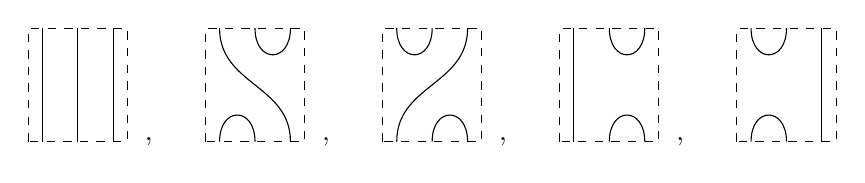
\begin{tikzpicture}[baseline=-1mm,scale=0.9]
		\pgfmathsetmacro{\yMax}{0.8};
		\pgfmathsetmacro{\offset}{2.5};
		\pgfmathsetmacro{\comma}{1};
		\foreach \x in {0,...,4}
			\draw[dashed] (-0.7+\offset*\x,-\yMax) rectangle (0.7+\offset*\x,\yMax);
		\begin{scope}[shift={(0,0)}]
			\foreach \x in {-0.5,0,0.5}
				\draw (\x, \yMax) -- (\x,-\yMax);
			\node (comma) at (+\comma,-\yMax) {$,$};
		\end{scope}
		\begin{scope}[shift={(1*\offset,0)}]
			\draw (0,\yMax) .. controls (0,-0.5+\yMax) and (0.5,-0.5+\yMax) .. (0.5,\yMax);
			\draw (-0.5,-\yMax) .. controls (-0.5,1-0.5-\yMax) and (0,1-0.5-\yMax) .. (0,-\yMax);
			\draw (-0.5,\yMax) .. controls (-0.5,0) and (0.5,0) .. (0.5, -\yMax);
			\node (comma) at (+\comma,-\yMax) {$,$};
		\end{scope}
		\begin{scope}[shift={(2*\offset,0)}]
			\draw (-0.5,\yMax) .. controls (-0.5,-0.5+\yMax) and (0,-0.5+\yMax) .. (0,\yMax);
			\draw (-0,-\yMax) .. controls (-0,1-0.5-\yMax) and (0.5,1-0.5-\yMax) .. (0.5,-\yMax);
			\draw (-0.5,-\yMax) .. controls (-0.5,0) and (0.5,0) .. (0.5, \yMax);
			\node (comma) at (+\comma,-\yMax) {$,$};
		\end{scope}
		\begin{scope}[shift={(3*\offset,0)}]
			\draw (-0.5,\yMax) -- (-0.5,-\yMax);
			\draw (0,\yMax) .. controls (0,-0.5+\yMax) and (0.5,-0.5+\yMax) .. (0.5,\yMax);
			\draw (-0,-\yMax) .. controls (-0,1-0.5-\yMax) and (0.5,1-0.5-\yMax) .. (0.5,-\yMax);
			\node (comma) at (+\comma,-\yMax) {$,$};
		\end{scope}
		\begin{scope}[shift={(4*\offset,0)}]
			\draw (0.5,\yMax) -- (0.5,-\yMax);
			\draw (-0.5,\yMax) .. controls (-0.5,-0.5+\yMax) and (0,-0.5+\yMax) .. (0,\yMax);
			\draw (-0.5,-\yMax) .. controls (-0.5,1-0.5-\yMax) and (0,1-0.5-\yMax) .. (0,-\yMax);
		\end{scope}
	\end{tikzpicture}
\,\,\right\}.
\end{align*}
We show how to perform multiplication:
\begin{align*}
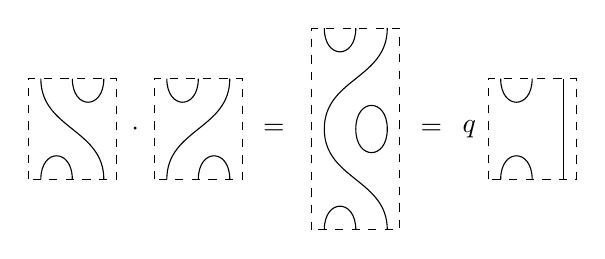
\begin{tikzpicture}[scale=0.8]
	\pgfmathsetmacro{\yMax}{0.8};
%
	\begin{scope}[shift={(0,0)}]
		\draw[dashed] (-0.7,-\yMax) rectangle (0.7,\yMax);
		\draw (0,\yMax) .. controls (0,-0.5+\yMax) and (0.5,-0.5+\yMax) .. (0.5,\yMax);
		\draw (-0.5,-\yMax) .. controls (-0.5,1-0.5-\yMax) and (0,1-0.5-\yMax) .. (0,-\yMax);
		\draw (-0.5,\yMax) .. controls (-0.5,0) and (0.5,0) .. (0.5, -\yMax);
		\node (comma) at (1,0) {$\cdot$};
	\end{scope}
	\begin{scope}[shift={(2,0)}]
		\draw[dashed] (-0.7,-\yMax) rectangle (0.7,\yMax);
		\draw (-0.5,\yMax) .. controls (-0.5,-0.5+\yMax) and (0,-0.5+\yMax) .. (0,\yMax);
		\draw (-0,-\yMax) .. controls (-0,1-0.5-\yMax) and (0.5,1-0.5-\yMax) .. (0.5,-\yMax);
		\draw (-0.5,-\yMax) .. controls (-0.5,0) and (0.5,0) .. (0.5, \yMax);
		\node (comma) at (1.2,0) {$=$};
	\end{scope}
 \begin{scope}[shift={(4.5,0)}]
	 	\draw[dashed] (-0.7,-2*\yMax) rectangle (0.7,+2*\yMax);
		\begin{scope}[shift={(0,-\yMax)}]
			\draw (0,\yMax) .. controls (0,-0.5+\yMax) and (0.5,-0.5+\yMax) .. (0.5,\yMax);
			\draw (-0.5,-\yMax) .. controls (-0.5,1-0.5-\yMax) and (0,1-0.5-\yMax) .. (0,-\yMax);
			\draw (-0.5,\yMax) .. controls (-0.5,0) and (0.5,0) .. (0.5, -\yMax);
		\end{scope}
		\begin{scope}[shift={(0,+\yMax)}]
			\draw (-0.5,+\yMax) .. controls (-0.5,-0.5+\yMax) and (0,-0.5+\yMax) .. (0,+\yMax);
			\draw (-0,-\yMax) .. controls (-0,1-0.5-\yMax) and (0.5,1-0.5-\yMax) .. (0.5,-\yMax);
			\draw (-0.5,-\yMax) .. controls (-0.5,0) and (0.5,0) .. (0.5, +\yMax);
		\end{scope}
		\node (comma) at (1.2,0) {$=$};
	\end{scope}
 \begin{scope}[shift={(7.3,0)}]
 		\node (q) at (-1,0) {$q$};
		\begin{scope}[shift={(0,0)}]
			\draw[dashed] (-0.7,-\yMax) rectangle (0.7,+\yMax);
			\draw (0.5,\yMax) -- (0.5,-\yMax);
			\draw (-0.5,\yMax) .. controls (-0.5,-0.5+\yMax) and (0,-0.5+\yMax) .. (0,\yMax);
			\draw (-0.5,-\yMax) .. controls (-0.5,1-0.5-\yMax) and (0,1-0.5-\yMax) .. (0,-\yMax);
		\end{scope}
	\end{scope}
\end{tikzpicture}.
\end{align*}
In the last step, we removed the circle and multiplied the result with $q$, then straightened the line and isotoped the box to give an element of $\mathcal{B}_3$. 

It is clear that $TL_3$ is closed under this multiplication.
\end{example}

There is no harm in not drawing the surrounding box, since we know that it is there. But omitting it makes drawing diagrams a lot faster, so we will do just that. We may simply write $TL_n$ for $TL_n(q)$ if $q$ is clear from context. In the following we will fix any $q$.

\bigno The elements in $TL_n$ are called \emph{$n$-tangles}, in anticipation of planar algebras. It is easy to see that the size of $\mathcal{B}_n$, which is the dimension of $TL_n$, is the same as the number of possible ways of putting matching opening and closing brackets on a product of $n+1$ factors, i.e.\ a product of $n$ pairs of factors, like this:
\begin{align*}
a((bc)d), \, a(b(cd)),\, (ab)(cd),\, ((ab)c)d,\, (a(bc))d
\end{align*}
Now, it would surely be nice to have a closed expression for this number, for any $n$. And indeed, this is a well-known problem from combinatorics. The solution is given by the \emph{Catalan numbers},
\begin{align*}
C_n \equiv\frac{1}{n+1} \binom{2n}{n}, n\geq 0.
\end{align*}
These numbers grow rather quickly:
\begin{align*}
	1, 1, 2, 5, 14, 42, 132, 429, 1430, 4862, 16796,\ldots\footnotemark
\end{align*}\footnotetext{This is sequence \emph{A000108} in the OEIS, see \url{oeis.org/A000108} for more interesting combinatorial interpretations.}
This makes calculating examples of perfect tangles particularly tedious, as we will argue in the coming chapters.

\bigno It is also worthwhile to briefly talk about another description of these algebras, namely the `classical' one in terms of generators and relations, see e.g.\ \cite{abramsky2009temperley}. Fix a ring $R$, a nonzero constant $q\in R$, and a natural number $n>1$. The Temperley-Lieb algebra on $n$ strands with loop value $q$ is then the unital associative algebra $A_n(q)$ over $R$ generated by the unit $1_A$ and generators $U_1, U_2,\ldots, U_{n-1}$ subject to the relations
\begin{alignat*}{2}
U_i^2 &= q\cdot U_i &&\\
U_i U_j U_i &= U_i &&\lvert i-j \rvert = 1\\
U_i U_j &= U_j U_i \qquad && \lvert i-j \rvert \geq 2
\end{alignat*}
Translating this into our previous description, we remark that the generators for $n=3$ are precisely the two last elements in $\mathcal{B}_3$ and the straight lines. For example,
\begin{align*}
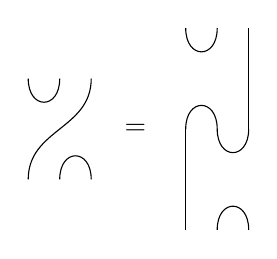
\begin{tikzpicture}[scale=0.8,baseline]
	\pgfmathsetmacro{\yMax}{0.8};
	\begin{scope}[shift={(0,0)}]
		\draw (-0.5,\yMax) .. controls (-0.5,-0.5+\yMax) and (0,-0.5+\yMax) .. (0,\yMax);
		\draw (-0,-\yMax) .. controls (-0,1-0.5-\yMax) and (0.5,1-0.5-\yMax) .. (0.5,-\yMax);
		\draw (-0.5,-\yMax) .. controls (-0.5,0) and (0.5,0) .. (0.5, \yMax);
		\node (comma) at (1.2,0) {$=$};
	\end{scope}
			\begin{scope}[shift={(2.5,-\yMax)}]
			\draw (-0.5,\yMax) -- (-0.5,-\yMax);
			\draw (0,\yMax) .. controls (0,-0.5+\yMax) and (0.5,-0.5+\yMax) .. (0.5,\yMax);
			\draw (-0,-\yMax) .. controls (-0,1-0.5-\yMax) and (0.5,1-0.5-\yMax) .. (0.5,-\yMax);
		\end{scope}
		\begin{scope}[shift={(2.5,\yMax)}]
			\draw (0.5,\yMax) -- (0.5,-\yMax);
			\draw (-0.5,\yMax) .. controls (-0.5,-0.5+\yMax) and (0,-0.5+\yMax) .. (0,\yMax);
			\draw (-0.5,-\yMax) .. controls (-0.5,1-0.5-\yMax) and (0,1-0.5-\yMax) .. (0,-\yMax);
		\end{scope}
\end{tikzpicture}\,.
\end{align*}
We record a following well-known fact, see e.g.\ \cite{kauffman1987state}.

\begin{fact}
Both descriptions of the Temperley-Lieb algebra given here are equivalent. In particular it can be shown that all crossingless matchings occurring in $\mathcal{B}_n$ can be obtained by multiplying diagrams consisting only of straight vertical lines, and cups and caps.
\end{fact}

